\documentclass[12pt,titlepage]{jarticle}

%\documentclass[12pt,titlepage]{article}
%\usepackage[whole]{bxcjkjatype}
%\setminchofont{ipaexm.ttf}
%\setgothicfont{ipaexg.ttf}

\usepackage{fancyhdr}
\usepackage{amsmath}
\usepackage{amssymb}
\usepackage{graphicx}
\usepackage{ascmac}
\usepackage{bm}% bold math
\usepackage{dcolumn}% Align table columns on decimal point
\usepackage{color}
\usepackage {framed,color}
%
%\pagestyle{fancy}
%
\topmargin=-30mm
\textheight=27cm
\textwidth=17cm
\oddsidemargin=-0.04 cm
\evensidemargin=-1.04cm
%1inchi = 2.54cm
%A4 = 21.0 * 29.7
%
\makeatletter
\renewenvironment{leftbar}{%
%  \def\FrameCommand{\vrule width 3pt \hspace{10pt}}%  デフォルトの線の太さは3pt
  \def\FrameCommand{\vrule width 1pt \hspace{0pt}}% 
  \MakeFramed {\advance\hsize-\width \FrameRestore}}%
 {\endMakeFramed}
\makeatother

\usepackage[T1]{fontenc}
\usepackage{xcolor}
\usepackage{lmodern}
\usepackage{listings}
\lstset{language=[90]Fortran,
  basicstyle=\ttfamily\small,
  keywordstyle=\color[rgb]{0,0,0.7},
  commentstyle=\color[rgb]{0.5,0,0},
  morecomment=[l]{!\ }% Comment only with space after !
}



\begin{document}
%
% Cover
%
\title{Shifted Krylov法ソフトウェア設計書 ver.0.1}
\author{東京大学物性研究所 ソフトウェア高度化推進チーム}
\date{\today}
\maketitle
%

%
% Contents
%
\tableofcontents

%%%%%%%%%%
\newpage
\section{概要}

本資料はKrylov部分空間法に基づくシフト線形方程式群ライブラリを用いたGreen関数計算用ソフトウェアに関する設計書である。
ライブラリに関する使用方法については、「Shifted Krylov法ライブラリ設計書」に記載した。

\subsection{ソフトウェア概要}
本ソフトウェアでは、Green関数
\begin{align}
  G_{i}(z) = \langle i | (z-{\hat H})^{-1}| i \rangle \equiv 
  {\boldsymbol \varphi}_i^{*} \cdot (z-{\hat H})^{-1} {\boldsymbol \varphi}_i
\end{align}
の計算を行う。ここで$| i \rangle $はベクトル、${\cal H}$はハミルトニアン、$z$は複素数である。\\
なお${\cal H}$については、
\begin{itemize}
\item{${\cal H}$をMatrixMarket形式の入力ファイルとして与えるモード}
\item{Heisenberg模型の${\cal H}$を内部で与えるモード}
\end{itemize}
を用意する。またグリーン関数の計算では、${\hat H}$と$z$が複素数もしくは実数かに応じ、
\begin{itemize}
\item ${\hat H}$も$z$も両方複素数の場合 : Shifted Bi-Conjugate Gradient(BiCG)法 or Shifted Conjugate Orthogonal Conjugate Gradient(COCG)法 
\item ${\hat H}$が実数で$z$が複素数の場合 : Shifted Conjugate Orthogonal Conjugate Gradient(COCG)法 
\item ${\hat H}$が複素数で$z$が実数の場合 : Shifted Conjugate Gradient(CG)法 (複素ベクトル)
\item ${\hat H}$も$z$も両方実数の場合 : Shifted Conjugate Gradient(CG)法 (実ベクトル)
\end{itemize}
の手法を用意する。デフォルトでは入力条件および入力ファイルからどのタイプかを自動判定し計算を行うものとする。ただし、各手法を手動で選択させ計算させることも可能とする。


\subsection{開発環境}
ver.1.0では並列化対応しないシンプルなものとする。
\begin{itemize}
\item{言語}\\
 Fortran90

 \item{使用ライブラリ}
 \begin{itemize}
 \item{Shifted Krylov法ライブラリ}
 \item{BLASレベル1ルーチン}
\end{itemize}

\end{itemize}

%%%%%%%%%%%%%%%%%%%%%%%%%
\newpage
\section{計算の流れ}
本ソフトウェアでは
\begin{enumerate}
\item{条件ファイルの読み込み}
\item{入力ファイルの読み込み (Hamiltonian, ベクトルなど)}
\item{リスタート用ファイルの読み込み (係数, 残差ベクトルなど)}
\item{ライブラリを利用したループ計算}
\item{計算結果ファイル出力(係数、残差ベクトル、動的グリーン関数)}
\end{enumerate}
の流れで計算を行う(図\ref{Fig:CalcFlow})。
使用の流れおよび各ファイルの詳細については、Sec. \ref{Sec:Usage}, \ref{Sec:FileFormat}にそれぞれ記載する。

\begin{figure}[htbp]
\begin{center}
	\includegraphics[width=12cm,clip]{KrylovSoft_ver.0.1.eps}
	\label{Fig:CalcFlow}
\end{center}
\end{figure}


%%%%%%%%%%%%%%%%%%%%%%%%%
\newpage
\section{使用の流れ}\label{Sec:Usage}
\subsection{Hamiltonian、ベクトルを読み込み計算する場合}
\subsubsection*{入力条件ファイルの作成}
周波数や計算時のループ回数の最大数などを指定するファイルを作成します。以下に入力ファイルの例を示します。\\
\begin{minipage}{10cm}
\begin{screen}
\begin{verbatim}
OmegaMax   10.0
OmegaMin  -10.0
OmegaIm    0.01
NOmega     100  
MaxLoops   2000
\end{verbatim}
\end{screen}
\end{minipage}
\\ \\
ここで\verb|OmegaMax|は$z$の実部の最大値、\verb|OmegaMin|は$z$の実部の最小値、\verb|OmegaIm|は$z$の虚部に対応します。\verb|NOmega|は動的グリーン関数を求めるための周波数$\omega_n = $ \verb|OmegaMin| $+n\times$(\verb|OmegaMax|-\verb|OmegaMin|)/\verb|NOmega| ($n=1\cdots$\verb|NOmega|)を指定するための変数です。また、\verb|MaxLoops|はループの最大数を指定します。省略可能な変数など、入力条件ファイルの詳細はSec. \ref{Sec:ModPara}を参照してください。

\subsubsection*{入力ファイルの作成}
MatrixMarket形式に従ったハミルトニアンの要素が記載されたファイルと励起ベクトルを記載したファイルを作成します。以下に励起ベクトルのファイル例を示します。\\
\\
\begin{minipage}{10cm}
\begin{screen}
\begin{verbatim}
# Re [v1]   Im[v1]
0.01    0.0
0.05    0.0
0.1     0.0
(continue ...)
\end{verbatim}
\end{screen}
\end{minipage}
\\\\
ファイル形式は \ref{subsubsec:ham},  \ref{subsubsec:vec}を参照してください。\\

\subsubsection*{入力ファイル指定ファイルの作成}
最初に入力ファイルのリストを記載したファイルを作成します。以下に入力ファイルの例を示します。\\
\begin{minipage}{10cm}
\begin{screen}
\begin{verbatim}
ModPara    modpada.def
InHam      Ham.dat
InVec      SingleExcitation.dat
\end{verbatim}
\end{screen}
\end{minipage}
\\\\
ここで\verb|ModPara|で紐付けられるファイルは動的グリーン関数を計算するために必要なパラメータ一式が定義されたファイル、
\verb|InHam|で紐付けられるファイルはMatrixMarket形式に従ったハミルトニアンの要素が記載されたファイル、
\verb|InVec|で紐付けられるファイルは励起ベクトルが記載されたファイルをそれぞれ指定するためのキーワードをそれぞれ表します。

\subsubsection*{計算実行}
作成した入力ファイル指定ファイルを引数にして計算実行します。
計算の途中経過は標準出力およびファイルでログ出力されます(\textcolor{red}{ログの内容に関しては要検討})。
ログファイルは自動生成される\verb|output|フォルダに格納されます。

以下、実行ファイルを\verb|ShiftK.out| 、入力ファイル指定ファイルを\verb|namelist.def|としてコマンド例を記載します。

\verb|$| \underline{パス}/\verb|ShiftK.out|  \verb|namelist.def|

\subsubsection*{計算結果出力}
以下のファイルが\verb|output|フォルダに出力されます。
\\
\begin{minipage}{11cm}
\begin{screen}
\begin{verbatim}
TriDiagComp.dat, ResVec.dat, dynamicalG.dat
\end{verbatim}
\end{screen}
\end{minipage}
\\ \\
ここで、
\verb|TriDiagComp.dat|はリスタート用の係数およびノルムが格納されているファイル、
\verb|ResVec.dat|はリスタート用の残差ベクトルが格納されているファイル、
\verb|dynamicalG.dat|は動的グリーン関数の計算結果が格納されているファイルをそれぞれ表します。
各ファイルのフォーマットはSec. \ref{subsubsec:ResVec}-\ref{subsubsec:DynamicalG}を参照ください。

%%%%%%%%%%%%%%%%%%%%%%%%%
\subsection{動的グリーン関数の再計算を行う場合}
動的グリーン関数を求めた際に出力される\verb|TriDiagComp.dat|および\verb|ResVec.dat|を用い、
異なる周波数での動的グリーン関数を再計算する場合の流れを示します。
\subsubsection*{入力条件ファイルの作成}
リスタート用のフラグ、周波数や計算時のループ回数の最大数などを指定するファイルを作成します。
以下に入力ファイルの例を示します。\\
\begin{minipage}{12.5cm}
\begin{screen}
\begin{verbatim}
# CalcType  0: normal (default), 1: recalc,  2: restart
CalcType   1          
OmegaMax   20.0
OmegaMin  -20.0
OmegaIm    0.005
NOmega     1000  
\end{verbatim}
\end{screen}
\end{minipage}
\\ \\
ここで\verb|OmegaMax|は$z$の実部の最大値、\verb|OmegaMin|は$z$の実部の最小値、\verb|OmegaIm|は$z$の虚部に対応します。\verb|NOmega|は動的グリーン関数を求めるための周波数$\omega_n = $ \verb|OmegaMin| $+n\times$(\verb|OmegaMax|-\verb|OmegaMin|)/\verb|NOmega| ($n=1\cdots$\verb|NOmega|)を指定するための変数です。{\bf \verb|CalcType|は計算モードを指定する変数で、再計算の場合には\verb|CalcType|の計算モードを$1$にする必要があります。}
また、\verb|MaxLoops|はループの最大数を指定します。省略可能な変数など、入力条件ファイルの詳細はSec. \ref{Sec:ModPara}を参照してください。

\subsubsection*{入力ファイル指定ファイルの作成}
最初に入力ファイルのリストを記載したファイルを作成します。以下に入力ファイルの例を示します。\\
\begin{minipage}{10cm}
\begin{screen}
\begin{verbatim}
ModPara    modpada.def
\end{verbatim}
\end{screen}
\end{minipage}
\\\\
ここで\verb|ModPara|で紐付けられるファイルは動的グリーン関数を計算するために必要なパラメータ一式が定義されたファイルを指定するためのキーワードを表します。

\subsubsection*{計算実行}
作成した入力ファイル指定ファイルを引数にして計算実行します。
\verb|output|フォルダにある\verb|TriDiagComp.dat|および\verb|ResVec.dat|を自動的に読み込まれます。
計算の途中経過は標準出力およびファイルでログ出力されます(\textcolor{red}{ログの内容に関しては要検討})。
ログファイルは自動生成される\verb|output|フォルダに格納されます。
なお、\verb|output|フォルダ内に\verb|dynamicalG.dat|が存在する場合は計算終了時に上書きされます。

以下、実行ファイルを\verb|ShiftK.out| 、入力ファイル指定ファイルを\verb|namelist.def|としてコマンド例を記載します。

\verb|$| \underline{パス}/\verb|ShiftK.out|  \verb|namelist.def|

\subsubsection*{計算結果出力}
\verb|output|フォルダ内にある\verb|dynamicalG.dat|が出力(同名のファイルが存在する場合には上書き)されます。

%%%%%%%%%%%%%%%%%%%%%%%%%
\subsection{リスタート計算をする場合}
\subsubsection*{入力条件ファイルの作成}
リスタート用のフラグ、周波数や計算時のループ回数の最大数などを指定するファイルを作成します。以下に入力ファイルの例を示します。\\
\begin{minipage}{12.5cm}
\begin{screen}
\begin{verbatim}
# CalcType  0: normal (default), 1: recalc,  2: restart
CalcType   2 
OmegaMax   10.0
OmegaMin  -10.0
OmegaIm    0.01
NOmega     100  
MaxLoops   2000
\end{verbatim}
\end{screen}
\end{minipage}
\\ \\
ここで\verb|OmegaMax|は$z$の実部の最大値、\verb|OmegaMin|は$z$の実部の最小値、\verb|OmegaIm|は$z$の虚部に対応します。\verb|NOmega|は動的グリーン関数を求めるための周波数$\omega_n = $ \verb|OmegaMin| $+n\times$(\verb|OmegaMax|-\verb|OmegaMin|)/\verb|NOmega| ($n=1\cdots$\verb|NOmega|)を指定するための変数です。また、\verb|MaxLoops|はループの最大数を指定します。{\bf \verb|CalcType|は計算モードを指定する変数で、リスタートの場合には\verb|CalcType|の計算モードを$2$にする必要があります。}
省略可能な変数など、入力条件ファイルの詳細はSec. \ref{Sec:ModPara}を参照してください。

\subsubsection*{入力ファイル指定ファイルの作成}
最初に入力ファイルのリストを記載したファイルを作成します。以下に入力ファイルの例を示します。\\
\begin{minipage}{10cm}
\begin{screen}
\begin{verbatim}
ModPara    modpada.def
InHam      Ham.dat
\end{verbatim}
\end{screen}
\end{minipage}
\\\\
ここで\verb|ModPara|で紐付けられるファイルは動的グリーン関数を計算するために必要なパラメータ一式が定義されたファイル、
\verb|InHam|で紐付けられるファイルはMatrixMarket形式に従ったハミルトニアンの要素が記載されたファイルでリスタート前に計算したものと同じファイルである必要があります。

\subsubsection*{計算実行}
作成した入力ファイル指定ファイルを引数にして計算実行します。
計算の途中経過は標準出力およびファイルでログ出力されます(\textcolor{red}{ログの内容に関しては要検討})。
ログファイルは自動生成される\verb|output|フォルダに格納されます。

以下、実行ファイルを\verb|ShiftK.out| 、入力ファイル指定ファイルを\verb|namelist.def|としてコマンド例を記載します。

\verb|$| \underline{パス}/\verb|ShiftK.out|  \verb|namelist.def|

\subsubsection*{計算結果出力}
以下のファイルが\verb|output|フォルダに出力されます。
\\
\begin{minipage}{11cm}
\begin{screen}
\begin{verbatim}
TriDiagComp.dat, ResVec.dat, dynamicalG.dat
\end{verbatim}
\end{screen}
\end{minipage}
\\ \\
ここで、
\verb|TriDiagComp.dat|はリスタート用の係数およびノルムが格納されているファイル、
\verb|ResVec.dat|はリスタート用の残差ベクトルが格納されているファイル、
\verb|dynamicalG.dat|は動的グリーン関数の計算結果が格納されているファイルをそれぞれ表します。
各ファイルのフォーマットはSec. \ref{subsubsec:ResVec}-\ref{subsubsec:DynamicalG}を参照ください。

%%%%%%%%%%%%%%%%%%%%%%%%%
\newpage
\section{ファイルフォーマット}\label{Sec:FileFormat}

\subsection{入力ファイル}
\subsubsection{入出力ファイル指定ファイル}
入力ファイルの種類と名前を指定します。各入力ファイルリストファイルでは、行毎にKeywordとファイル名を記載し、ファイルの種類の区別を行います。\\
\begin{minipage}{15cm}
\begin{screen}
\begin{verbatim}
ModPara modpara.def
InHam   Hamiltonianl.dat
Invec   vec.dat
\end{verbatim}
\end{screen}
\end{minipage}
\\

\subsubsection{ファイル形式}
[string01]~[string02]
\subsubsection{パラメータ}
 \begin{itemize}
   \item  $[$string01$]$
   
   {\bf 形式 :} string型 (固定)
   
   {\bf 説明 :} キーワードを指定します。
   
   \item  $[$string02$]$
   
    {\bf 形式 :} string型 

   {\bf 説明 :} キーワードにひも付けられるファイル名を指定します(任意)。
 \end{itemize}
 
\subsubsection{使用ルール}
本ファイルを使用するにあたってのルールは以下の通りです。
\begin{itemize}
\item キーワードを記載後、半角空白を開けた後にファイル名を書きます。ファイル名は自由に設定できます。
\item ファイル読込用キーワードはTable\ref{Table:Defs}により指定します。
\item 必ず指定しなければいけないパラメーターは\verb|ModPara|です。
\item 各キーワードは順不同に記述できます。
\item 指定したキーワード、ファイルが存在しない場合はエラー終了します。
\item $\#$で始まる行は読み飛ばされます。
\end{itemize}

 \begin{table*}[h!]
\begin{center}
  \begin{tabular}{ll|} \hline
           ModPara       &  計算に必要なパラメータ一式を指定するファイル指定用。        \\ \hline   
           InHam        &   入力するハミルトニアンのファイル指定用。          \\   
           InVec         &   入力する励起ベクトルファイル指定用。 \\   \hline
  \end{tabular}
\end{center}
\caption{ファイル名を指定するキーワード一覧}
\label{Table:Defs}
\end{table*}%

\subsection{ModParaファイル}
\label{Subsec:modpara}
計算で使用するパラメータを指定します。以下のようなフォーマットをしています。\\
\begin{minipage}{10cm}
\begin{screen}
\begin{verbatim}
OmegaMax   10.0
OmegaMin  -10.0
OmegaIm    0.01
NOmega     100  
MaxLoops   2000
\end{verbatim}
\end{screen}
\end{minipage}

\subsubsection{ファイル形式}
[string01]~[int01/double01]

\subsubsection{パラメータ}
\begin{itemize}
   \item  $[$string01$]$
   
   {\bf 形式 :} string型 (固定)

  {\bf 説明 :} キーワードの指定を行います。
   
   \item  $[$int01$]$
   
   {\bf 形式 :} int型 (空白不可)

  {\bf 説明 :} キーワードで紐付けられるパラメータを指定します。

   \item  $[$double01$]$
   
   {\bf 形式 :} double型 (空白不可)

  {\bf 説明 :} キーワードで紐付けられるパラメータを指定します。

 \end{itemize}

\subsubsection{使用ルール}
本ファイルを使用するにあたってのルールは以下の通りです。
\begin{itemize}
\item キーワードを記載後、半角空白を開けた後に数値を書きます。
\end{itemize}

~\subsubsection{キーワード}
 \begin{itemize}
  \item  \verb|MakeHam|

 {\bf 形式 :} int型 (デフォルト値 0)

{\bf 説明 :} 
Hamiltonianの読み込みの有無を指定するキーワード(ver. 1.0では常に読み込むため$0$が自動指定)。
\begin{itemize}
\item{0: ハミルトニアン読み込みあり。}
\item{1: ハミルトニアン読み込みなし。}
\end{itemize}
   
 \item  \verb|OmegaMax|

{\bf 形式 :} double型 (空白不可)

{\bf 説明 :} 計算対象となる振動数$\omega$の実部の最大値を指定する実数。  

\item  \verb|OmegaMin|

{\bf Type :} {double型 (空白不可)}

{\bf 説明 :} 計算対象となる振動数$\omega$の実部の最小値を指定する実数。  

 \item  \verb|OmegaIm|

{\bf Type :} {double 型 (デフォルト値 0)}

{\bf 説明:} {計算対象となる振動数$\omega$に加えられる虚部を指定する実数。}

 \item  \verb|OmegaSeed|

{\bf Type :} {double 型 (デフォルト値 0)}

{\bf 説明:} {シード振動数$\omega$を与える実数。}

 \item  \verb|OmegaImMax|

{\bf 形式 :} double型 (空白不可)

{\bf 説明 :} 計算対象となる振動数$\omega$の虚部の最大値を指定する実数。  

\item  \verb|OmegaImMin|

{\bf Type :} {double型 (空白不可)}

{\bf 説明 :} 計算対象となる振動数$\omega$の虚部の最小値を指定する実数。  


 \item  \verb|NOmega|

{\bf 形式 :} int型 (自然数)

{\bf 説明 :} 計算対象となる振動数$\omega$を指定する整数。計算対象となる振動数は$\omega_{\rm max}$と$\omega_{\rm min}$を\verb|NOmega|分割した振動数で与えられます。

 \item  \verb|MaxLoops|

{\bf 形式 :} int型 (自然数、デフォルト値 1000)

{\bf 説明 :} 計算内で残差ベクトルをアップデートする最大数を指定します。
指定した精度内で収束した場合には、これより短い回数で終了します。

 \item  \verb|ConvFactor|

{\bf 形式 :} int型 (自然数)

{\bf 説明 :}  残差ベクトルを評価するためのファクター。 \verb|ConvFactor|$=\eta$として$10^{-\eta}$で与えます。

\item  \verb|OutRestart|

{\bf 形式 :} int型 (自然数、デフォルト値は0)

{\bf 説明 :} 
\begin{itemize}
\item{0: リスタート用ファイル出力なし。}
\item{1: リスタート用ファイル出力あり。}
\end{itemize}


 \item  \verb|CalcType|

{\bf 形式 :} int型 (整数)

{\bf 説明 :} 
\begin{itemize}
\item{0: 通常計算。}
\item{1: 振動数を変えた再計算。}
\item{2: リスタートなし。}
\end{itemize}


\end{itemize}
  
\newpage
\subsubsection{InHamファイル} \label{subsubsec:ham}
MatrixMarket形式に準ずる。

\subsubsection{InVecファイル}\label{subsubsec:vec}
励起ベクトルを入力するテキスト形式のファイルです。ファイル名は入出力ファイル指定ファイルで指定します。
以下のようなフォーマットをしています。
\\
\begin{minipage}{10cm}
\begin{screen}
\begin{verbatim}
8192
0.02 0.01
0.02 0.001
(continue...)
\end{verbatim}
\end{screen}
\end{minipage}


\subsubsection{ファイル形式}
 \begin{itemize}
   \item  1行目:$[$int01$]$
   \item  2行目-: $[$double01$]$~~$[$double02$]$
  \end{itemize}
\subsubsection{パラメータ}
 \begin{itemize}

  \item  $[$int01$]$

 {\bf 形式 :} int型

{\bf 説明 :} 計算対象のヒルベルト空間数を指定する整数。
 
 \item  $[$double01$]$, $[$double02$]$

 {\bf 形式 :} double型 

{\bf 説明 :} 励起ベクトルの値を表します。\\
$[$double01$]$が実部、$[$double02$]$が虚部を表します。\\
\end{itemize}


\newpage
\subsubsection{リスタート用係数}\label{subsubsec:recoeff}
リスタート用の係数を入力するテキスト形式のファイルです。ファイル名は入出力ファイル指定ファイルで指定します。
以下のようなフォーマットをしています。
\\
\begin{minipage}{10cm}
\begin{screen}
\begin{verbatim}
1000
0.1 0 0.01  0
0.2 0 0.021 0
(continue...)
\end{verbatim}
\end{screen}
\end{minipage}


\subsubsection{ファイル形式}
 \begin{itemize}
   \item  1行目:$[$int01$]$
   \item  2行目-: $[$double01$]$~~$[$double02$]$~~$[$double03$]$~~$[$double04$]$
  \end{itemize}
\subsubsection{パラメータ}
 \begin{itemize}

  \item  $[$int01$]$

 {\bf 形式 :} int型

{\bf 説明 :} $\alpha, \beta$の読み込み総数を表します。前回計算時のイタレーション数に相当します。
 
 \item  $[$double01$]$, $[$double02$]$, $[$double03$]$, $[$double04$]$

 {\bf 形式 :} double型 

{\bf 説明 :} $\alpha, \beta$の値を表します。\\
$[$double01$]$が$\alpha$の実部、$[$double02$]$が$\alpha$の虚部、
$[$double03$]$が$\beta$の実部、$[$double04$]$が$\beta$の虚部を表します。\\
\end{itemize}


\newpage
\subsubsection{リスタート用ベクトル}\label{subsubsec:revec}
リスタート用ベクトルを入力するテキスト形式のファイルです。ファイル名は入出力ファイル指定ファイルで指定します。
以下のようなフォーマットをしています。
\\
\begin{minipage}{10cm}
\begin{screen}
\begin{verbatim}
8192
0.02 0.01
0.02 0.001
(continue...)
\end{verbatim}
\end{screen}
\end{minipage}


\subsubsection{ファイル形式}
 \begin{itemize}
   \item  1行目:$[$int01$]$
   \item  2行目-: $[$double01$]$~~$[$double02$]$
  \end{itemize}
\subsubsection{パラメータ}
 \begin{itemize}

  \item  $[$int01$]$

 {\bf 形式 :} int型

{\bf 説明 :} 計算対象のヒルベルト空間数を指定する整数。
 
 \item  $[$double01$]$, $[$double02$]$

 {\bf 形式 :} double型 

{\bf 説明 :} ベクトルの値を表します。\\
$[$double01$]$が実部、$[$double02$]$が虚部を表します。\\
\end{itemize}


\newpage
\subsection{出力ファイル}
\subsubsection{リスタート用係数}\label{subsubsec:ResCoef}
\ref{subsubsec:recoeff}と同じ形式を取る。
\subsubsection{リスタート用ベクトル}\label{subsubsec:ResVec}
\ref{subsubsec:revec}と同じ形式を取る。
\subsubsection{動的グリーン関数ファイル}\label{subsubsec:DynamicalG}

動的グリーン関数の計算結果を出力するテキスト形式のファイルです。
以下のようなフォーマットをしています。
\\
\begin{minipage}{10cm}
\begin{screen}
\begin{verbatim}
-10 0.001 0.001 -0.0001 
-9.8 0.001 0.0012 -0.0002
-9.6 0.001 0.0014 -0.0003
(continue...)
\end{verbatim}
\end{screen}
\end{minipage}


\subsubsection{ファイル形式}
 \begin{itemize}
   \item 1行目-: $[$double01$]$~~$[$double02$]$~~$[$double03$]$~~$[$double04$]$
  \end{itemize}
\subsubsection{パラメータ}
 \begin{itemize}

  \item  $[$double01$]$,$[$double02$]$

 {\bf 形式 :} double型

{\bf 説明 :} 周波数数の実部 $[$double01$]$と虚部$[$double02$]$を表します。
 
 \item  $[$double03$]$, $[$double04$]$

 {\bf 形式 :} double型 

{\bf 説明 :} 動的グリーン関数の値を表します。\\
$[$double01$]$が実部、$[$double02$]$が虚部を表します。\\
\end{itemize}

\end{document}
